\documentclass[a4paper]{jarticle}
\usepackage{amsmath}
\usepackage[dvipdfmx]{graphicx}
\usepackage[dvipdfmx]{color}

\setlength{\textheight}{244truemm}
\setlength{\headheight}{0pt}
\setlength{\headsep}{25truemm}
\setlength{\footskip}{15truemm}
\addtolength{\topmargin}{-1truein}
\setlength{\textwidth}{145truemm}
\setlength{\oddsidemargin}{35truemm}
\addtolength{\oddsidemargin}{-1truein}

\begin{document}
	\section{目的}
		抵抗($R$)とコイル($L$)の直列接続回路の電圧・電流を測定し、回路のインピーダンス・電流・位相について理解する。
	\section{理論}
		抵抗$R$ [Ω]とコイル$L$ [H]の直列接続回路は、交流に対して電流の流れを妨げる働きをする。
		これをインピーダンスという。RL直列回路のインピーダンス$Z$ [Ω]は、$R$と誘導性リアクタンス$X_{L}$との代数和にならず、
		次式で表される。
		\begin{flalign}
			Z & = \sqrt{R^{2} + \left(X_{L}\right)^{2}} \nonumber &\\
			   & = \sqrt{R^{2} + \left(ωL\right)^{2}}
		\end{flalign}
		また、交流電源の電圧を$v$ [V]、RL直列回路を流れる電流を$i$ [A]とすると、
		\begin{flalign}
			i & = \frac{v}{Z} \qquad[\mathrm{A}] &
		\end{flalign}
		となる。
		\begin{figure}[h]
			\begin{minipage}{0.5\hsize}
				\begin{center}
					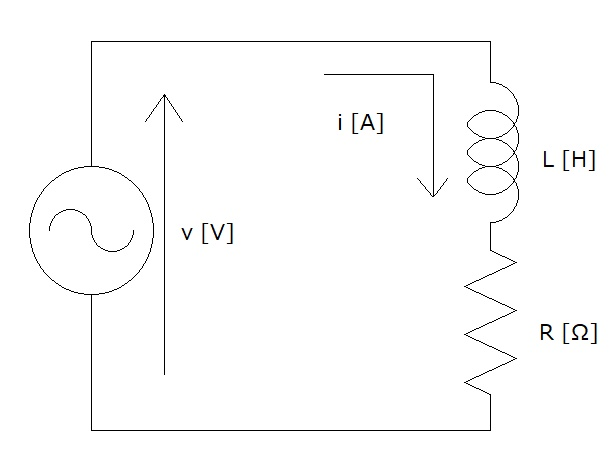
\includegraphics[width = 5cm]{RL直列回路と交流図1.jpg}
				\end{center}
				\caption{RL直列回路}
			\end{minipage}
			\begin{minipage}{0.5\hsize}
				\begin{center}
					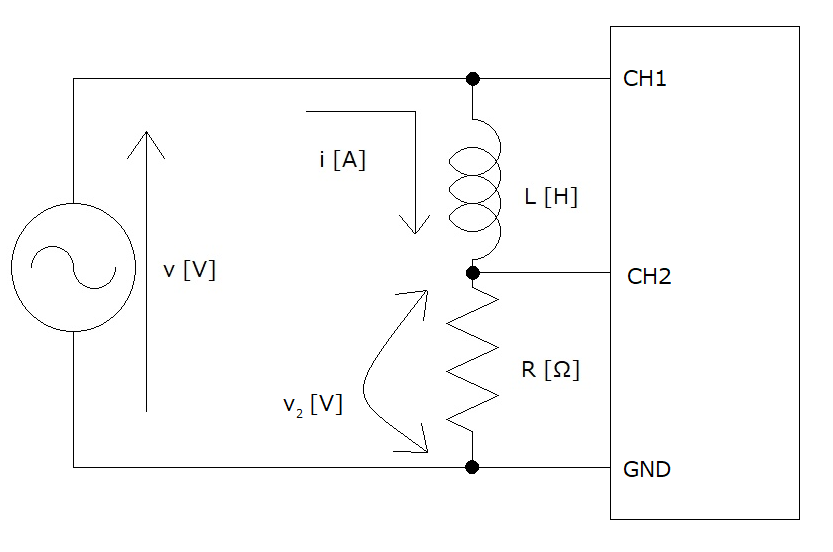
\includegraphics[width = 7cm]{RL直列回路と交流図2.jpg}
				\end{center}
				\caption{RL直列回路}
			\end{minipage}
		\end{figure}
	\section{実験}
		\subsection{原理}
			\subsubsection{電流の大きさ}
				RL直列回路に流れる電流は$R$を利用して測定する。図2においてRL直列回路を流れる電流は、$R$をも流れている。
				したがって、$R$の両端の電圧$v_{2}$ [V]を測定し、$R$ [Ω]で割れば、$R$を流れる電流$i_{R}$すなわち、
				$i$がわかる。
				\begin{flalign}
					i_{R} & = \frac{v_{2}}{R} &\\
					i & = i_{R} \nonumber
				\end{flalign}
			\subsubsection{電圧と電流の位相差}
				2つ以上の交流波形の時間的なずれを位相差と呼ぶ。位相差は交流波形の1周期を角度(360°または2π)に換算し、表現する。\par
				図3を例にとると、$V$に比べ、$I$は右側にちょうど1目盛分ずれている。1周期4目盛を360°として、ずれは1目盛分なのだから、
				$V$に対する$I$の位相差は次のように計算できる。
				\begin{flalign}
					\frac{360°}{4} × 1 & = 90° \nonumber&
				\end{flalign}\par
				一般に、$V$と$I$の関係のように$V$に比べ$I$が右側にある状態を、\\
				\qquad$I$は$V$に比べ、90°遅れている\\
				と表現する。
				\begin{figure}[h]
					\begin{center}
						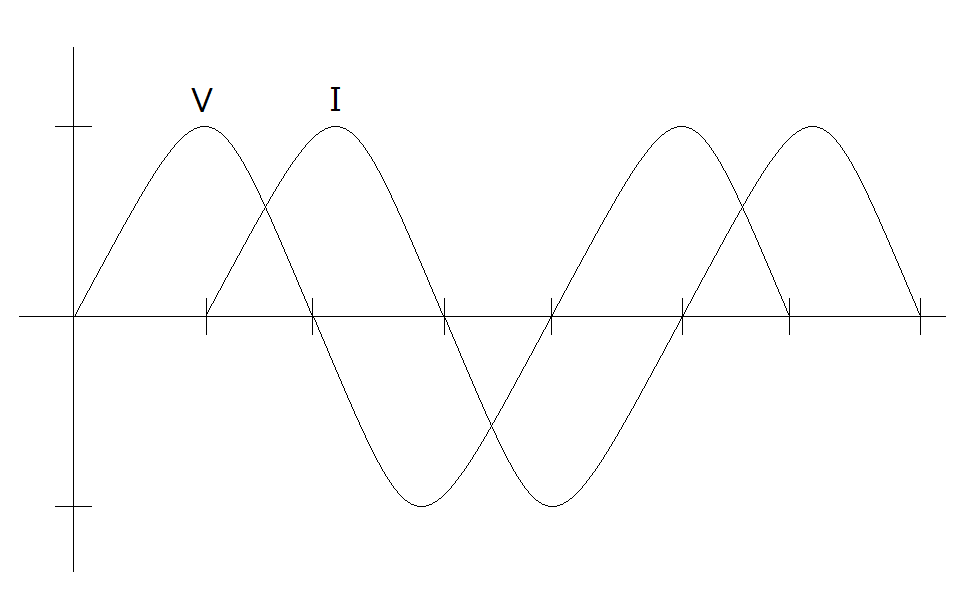
\includegraphics[width = 10cm]{RL直列回路と交流図3.jpg}
					\end{center}
					\caption{電圧($V$)と電流($I$)との位相差}
				\end{figure}
		\subsection{コイルの電圧と電流の位相差}
			コイルだけの回路で、コイルの電圧に対するコイルを流れる電流の位相差について測定する。図2の接続図で、$R$の値を$X_{L}$に比べて、
			無視できるぐらい小さな値にすると、コイルだけの回路と考えることができる。
			\subsubsection{測定}
				\begin{enumerate}
					\item[(ア)]{図2のように接続する。}
					\item[(イ)]{抵抗 $R = 10$ [Ω]}
					\item[(ウ)]{コイル $L = 50$ [mH]}
				  \item[(エ)]{交流電圧 $V = 2.83$ [Vrms]}
					\item[(オ)]{$f = 1$ [kHz]}
					\item[(カ)]{$f = 1 \ [\mathrm{kHz}] ~ 10 \ [\mathrm{kHz}]、1 \ [\mathrm{kHz}]$間隔}
					\item[(キ)]{コイルの電圧波形$v$、コイルの電流波形$v_{2}$、として位相差を測定する。}
				\end{enumerate}
			\subsubsection{測定結果}
				\begin{table}[h]
					\centering
					\small
					\caption{コイルの電圧と電流の位相差}
					\begin{tabular}{c|c|c|c|c}\hline\hline
						周波数 [kHz] & 1周期 [目盛] & ずれ [目盛] & 位相差 [°] & コイルの電圧対する電流の遅れ・進み \\ \hline
						1 & 4.0 & 1.0 & 90 & 遅れている \\
						2 & 5.0 & 1.2 & 86 & 遅れている \\
						3 & 3.4 & 0.9 & 95 & 遅れている \\
						4 & 5.0 & 1.2 & 86 & 遅れている \\
						5 & 4.0 & 1.0 & 90 & 遅れている \\
						6 & 3.4 & 0.8 & 85 & 遅れている \\
						7 & 5.7 & 1.5 & 95 & 遅れている \\
						8 & 5.0 & 1.9 & 86 & 遅れている \\
						9 & 4.5 & 1.1 & 88 & 遅れている \\
						10 & 4.0 & 1.0 & 90 & 遅れている \\ \hline
					\end{tabular}
				\end{table}
		\subsection{RL直列回路の電流・インピーダンス・位相差測定}
			\subsubsection{測定}
				\begin{enumerate}
					\item[(ア)]{図2のように接続する。}
					\item[(イ)]{抵抗 $R = 1000$ [Ω]}
					\item[(ウ)]{コイル $L = 50$ [mH]}
				  \item[(エ)]{交流電圧 $V = 2.83$ [Vrms]}
					\item[(オ)]{$f = 1$ [kHz]}
					\item[(カ)]{$f = 1 \ [\mathrm{kHz}] ~ 10 \ [\mathrm{kHz}]、1 \ [\mathrm{kHz}]$間隔で、抵抗の電圧$v_{2} \ [\mathrm{Vrms}]$、
					位相差を測定する。}
					\item[(キ)]{測定結果から、電流$i$ [Arms]、インピーダンス$Z$ [Ω]を算出する。}
				\end{enumerate}
			\subsubsection{測定結果}
				\begin{table}[h]
					\centering
					\small
					\caption{RL直列回路の電流・インピーダンス・位相差}
					\begin{tabular}{c|c|c|c|c|c|c|c|c|c}\hline\hline
						 & \multicolumn{2}{c|}{計算結果} & \multicolumn{7}{c}{測定結果} \\ \cline{2-10}
						\multicolumn{1}{c|}{周波数} & & &\multicolumn{3}{c|}{電流・インピーダンス} & \multicolumn{4}{c}{位相差} \\ \cline{4-10}
						[kHz] & $i$ [mA] & $Z$ [kΩ] & $v_{2}$ & $i$ & $Z$ & 1周期 & ずれ  & 位相差 & コイルの電圧対する \\
						 & & & [V] & [mA] & [kΩ] & [目盛] & [目盛] & [°] & 電流の遅れ・進み \\ \hline
						1 & 2.7 & 1.1 & 3.8 & 3.8 & 0.74 & 4.0 & 0.2 & 18 & 遅れている \\
						2 & 2.4 & 1.2 & 3.6 & 3.6 & 0.79 & 5.0 & 0.5 & 36 & 遅れている \\
						3 & 2.1 & 1.4 & 2.8 & 2.8 & 1.0 & 3.4 & 0.4 & 42 & 遅れている \\
						4 & 1.8 & 1.6 & 2.4 & 2.4 & 1.2 & 5.0 & 0.7 & 50 & 遅れている \\
						5 & 1.5 & 1.9 & 2.1 & 2.1 & 1.4 & 4.0 & 0.6 & 54 & 遅れている \\
						6 & 1.3 & 2.1 & 1.9 & 1.9 & 1.5 & 6.7 & 1.2 & 65 & 遅れている \\
						7 & 1.2 & 2.4 & 1.7 & 1.7 & 1.7 & 5.7 & 1.1 & 70 & 遅れている \\
						8 & 1.0 & 2.7 & 1.5 & 1.5 & 1.9 & 5.0 & 1.0 & 72 & 遅れている \\
						9 & 0.94 & 3.0 & 1.4 & 1.4 & 2.0 & 4.4 & 0.9 & 74 & 遅れている \\
						10 & 0.86 & 3.3 & 1.2 & 1.2 & 2.4 & 4.0 & 0.8 & 72 & 遅れている \\ \hline
					\end{tabular}
				\end{table}
	\section{使用器具}
		発振器: L151-1-73 \par
		コイル: E111-3-13 \par
		抵抗: M97-462 \par
		オシロスコープ: DSO NO.7
	\section{課題・考察}
		\begin{enumerate}
			\item[1.]{3.2.2の測定結果から、周波数対位相差をグラフで表せ。}
				\begin{figure}[h]
					\begin{center}
						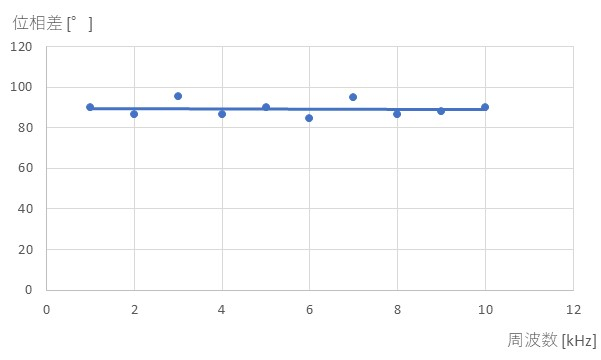
\includegraphics[width = 7cm]{RL直列回路と交流グラフ1.jpg}
					\end{center}
					\caption{周波数対位相差グラフ}
				\end{figure}
			\item[2.]{3.3.2の測定結果から、周波数対インピーダンス、周波数対操作をグラフで表せ。}
				\begin{figure}[h]
					\begin{minipage}{0.5\hsize}
						\begin{center}
							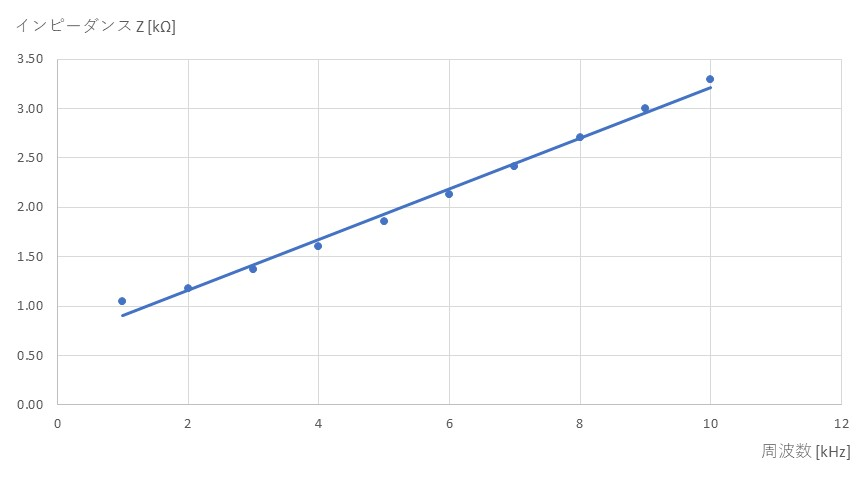
\includegraphics[width = 7cm]{RL直列回路と交流グラフ2.jpg}
						\end{center}
						\caption{周波数対インピーダンスグラフ}
					\end{minipage}
					\begin{minipage}{0.5\hsize}
						\begin{center}
							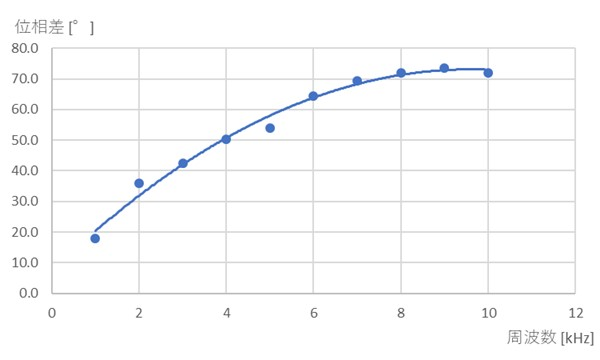
\includegraphics[width = 7cm]{RL直列回路と交流グラフ3.jpg}
						\end{center}
						\caption{周波数対位相差グラフ}
					\end{minipage}
				\end{figure}
			\item[3.]{3.2.2の測定結果から、コイルの電圧とコイルを流れる電流について言えることは何か。教科書等を参考に述べよ。} \\
				コイルを流れる電流$i$は電圧$v$より90 [°]だけ位相が遅れている。
			\item[4.]{3.3.2の測定結果において、電流の大きさ、インピーダンスについて、計算値と測定結果を比較せよ。} \\
				電流は、測定結果が計算結果の$\sqrt{2}$倍で、インピーダンスは逆の結果になっている。これは、測定は交流で行っているため、
				電圧の値は実測値であるが、計算で使っている電圧値は最大値であるためだと考えられる。実際に、すべて最大値として計算をした場合、
				二つの値の差はほとんど誤差となる。
		\end{enumerate}
\end{document}
